\chapter{Ma contribution: replication mais avec MEG}

% Setup
% - renvoyer au document de l'ensemble des choses que j'auraient aimés savoir dés le début

% Deux études : 
% - Welcome study
% - Localizer ?
% - Sample

\section{Preprocessing}

La différence entre les travaux que j'avais déjà fait lors du cours du MVA Imagerie fonctionnelle cerebrale pour le challenge Kaggle BCI et ce cours repose surtout sur le fait que la donnée à travaité a deja été nettoyé lors du challenge Kaggle. Même si le nettoyage de la donnée n'était pas le coeur de mon stage, il a fallut y poaaser un temps consequent.

Les différentes phases du preprocessing de la données se fait comme suit:


The common preprocessing steps of raw MEG data are the following:
\begin{itemize}
    \item Finding bad channels: some channels of MEG recordings may be noisy or flat. They need to be identified and marked as bad so they are not taking into account during the analysis;
    \item Applying Maxwell filter : help to remove part of the sensors noise;
    \item Frequency filter: to remove non desired frequency bands;
    \item Creating epochs: epochs are data structures to represent equal-duration chuncks of MEG
          signals. When the recording session includes stimuli, epochs are often defined from 0.2 seconds
          before the stimulus to 0.5 seconds after. Otherwise, like in rest session, epochs are fixed and
          overlapping frames of the MEG signal.
    \item Computing evoked data: they are created by averaging MEG signal over several epochs. It is useful to study stimulus-evoked brain activity.
\end{itemize}


La figure \ref{cheat_sheet} resume l'étape du preprocessing dans la pipeline

\begin{figure}[ht]
    \centering
    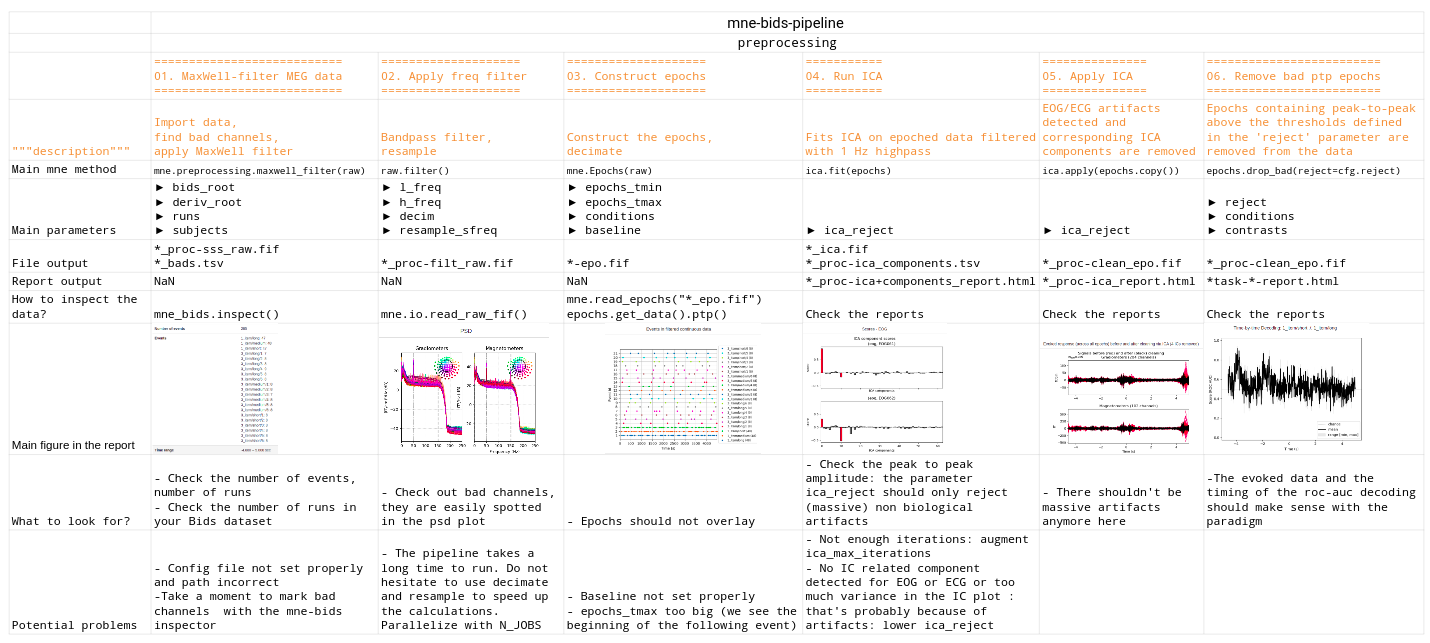
\includegraphics[width=15cm]{images_report/preprocessing/cheatsheet preprocessing.png}
    \caption[sheat sheet of the preprocessing of the pipeline]%
    {sheat sheet of the preprocessing of the pipeline}

    \label{cheat_sheet}
\end{figure}


\subsection{Bids Pipeline}
- Premiereres PR necessité pourquoi ?
premiere contri open source
avec une utilité

Lors de l'étape du preprocessing au début de mon stage, il a fallut que je me familiarise avec la librairie mne-bids-pipeline et tous ses différents script, et également afin de me familieariser avec le developpement open-source ainsi que les exigences qui en découlent.

Mes premieeres contributions consistere donc à rajouter des sanity check dans la pipeline, actualiser les docstring et les en tetes de codes, travailler sur l'hormonie du code en harminisant les noms des variables entre les différents scripts.

\subsection{Preprocessing of artifacts}


\begin{figure}[ht]
    \centering
    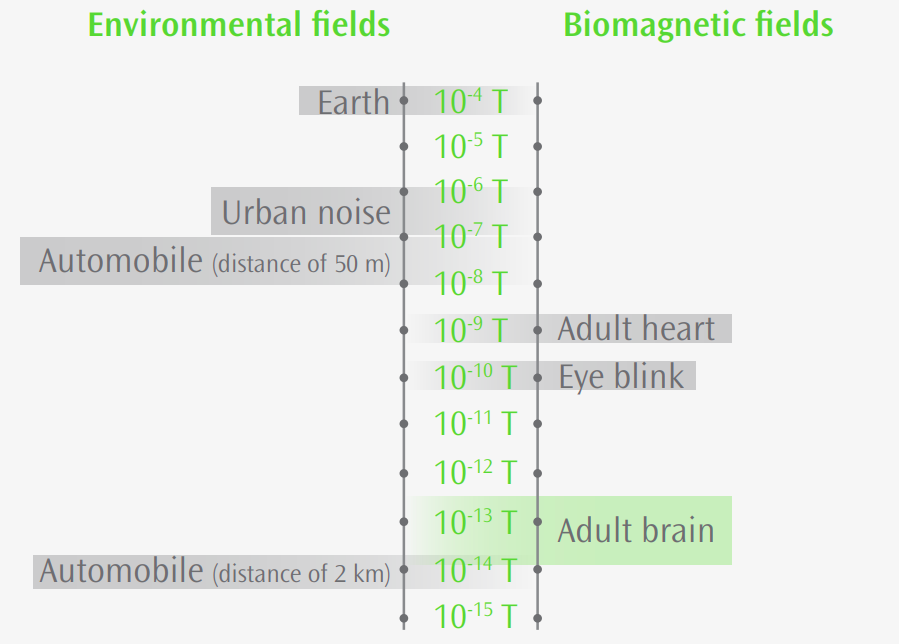
\includegraphics[width=7cm]{images_report/sensor/noise_order_of_magnitude.png}
    \caption[Scale of magnitude of different magnetic fields]%
    {Scale of magnitude of different magnetic fields}

    \label{noise_order_of_magnitude}
\end{figure}


Apres m'être familiarisé avec la l'esprit du code, j'ai pu travailler sur la logique. Notemment un point important qui est l'ordre dans lequel la donnée est rejetée. En effet, une difficulté majeure des données brutes venant des signaux corticaux est le fait que ces signaux sont minuscules. Bien que l'enregistrement des donnée se fassent dans une chambre blindée, le moindre bruit peut ecraser totalement le signal. La figure \ref{noise_order_of_magnitude} présente l'échelle des ordres de grandeurs, qui montre bien que les bruits exterieux sont d'un ordre de granduer incommensurablement plus grands que les signaux d'interets neurologiques.

Même apres avoir enlevé tous les bruits venant de l'environnement exterieur certains bruits que l'on appelle artifacts biologiques, tels que les battement de coeurs ou bien les clignement d'oeils doivent être soit enlevés en rejetant l'interval temporel contaminé, soit en sépanrant les sources par l'usage de l'analyse en composante indépandantes (ICA), qui permet de séparer les ssources de signaux emises par le coeurs ou les clignements d'oeuil du reste du signal.

La figure \ref{rejection_pipeline} permet visualiser la rejection pipeline de la mne-bids-pipeline.

\begin{figure}[ht]
    \centering
    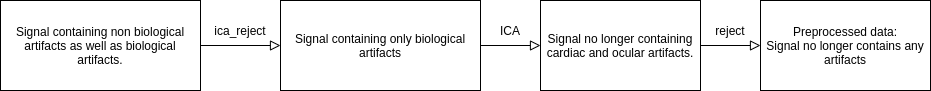
\includegraphics[width=15cm]{images_report/preprocessing/rejection_pipeline.png}
    \caption[Simplification of the rejection pipeline of the bids pipeline.]%
    {Simplification of the rejection pipeline of the bids pipeline.}
    \label{rejection_pipeline}
\end{figure}

Voici le détail de la procédure:
\begin{itemize}
    \item Au début le signal contient des artefacts à la fois biologiques (clignement d'oeil, battement de coeur), et non biologiques. Ces derniers sont d'un ordre de grandeur d'amplitude plus grands que les artefacts biologiques.
    \item On peut commencer par filtrer les différentes epoches en utilisant rejetant les epochs dnt l'amplitude peak-to-peak dépasse l'amplitude specifiée par le parametre "ica\_reject". Ce parametre permet de filtrer des signaux qui en ordre de grandeur sont 50 fois plus grand qu'une amplitude nominale et permet donc de faire un premier tris.
    \item Le signal resultant ne contient plus d'artefact non biologique redhibitoire, ce qui peremt d'améliorer la convergence de l'ICA, qui permet de séparer les sources pour les artefacts oculaires et cardiques.
    \item La séparation de source par ICA ne fonctionne pas parfaitement, et il faut donc prevoir une étape supplémentaire afin de rejeter les derniers artefacts à l'aide du parametere "reject", qui permet de filter les signaux avec une amplitude peak-to-peak 10 fois supérieure à l'amplitude nominale. On obtient alors le signal preprocessed.
\end{itemize}

Même si la méthode globale de rejection de la pipeline était déjà établie avznt mon arivée, les donées experiementales ont revelées des problemes dans l'ordre des opération de filtrage, et nous avons aisi amélioré de beaucoup le preprocessing automatique de la donnée notemment pour de la donnée difficile qui contient simulanément des artifacts biologique et des artifacts non-biologiques telles que des inversion de champs de phase. La figure \ref{fig:PR_ica} montre un example d'amélioration des ICA.



\begin{figure}
    \centering
    \begin{subfigure}{.5\textwidth}
        \centering
        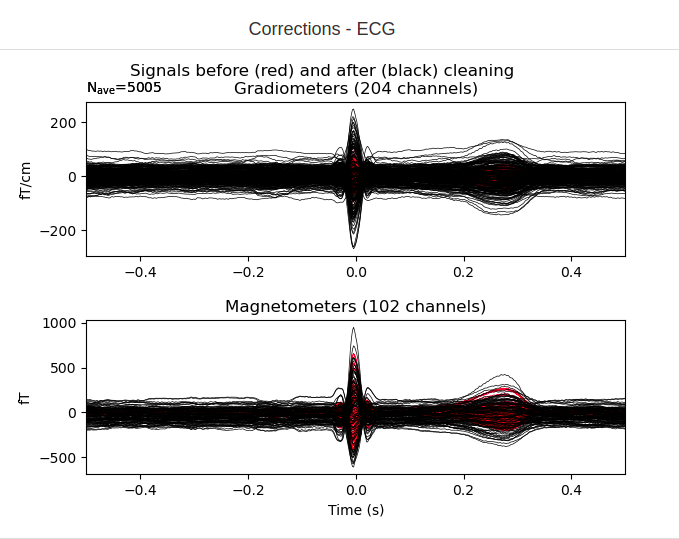
\includegraphics[width=1.\linewidth]{images_report/preprocessing/ica/ECG_ICA_before_PR.png}
        \caption{ICA correction before amelioration}
        \label{fig:before_ica_PR}
    \end{subfigure}%
    \begin{subfigure}{.5\textwidth}
        \centering
        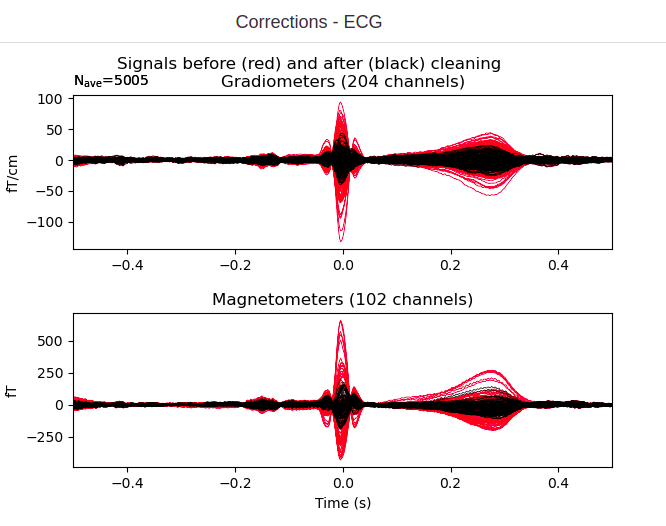
\includegraphics[width=1.\linewidth]{images_report/preprocessing/ica/ECG_ICA_after_PR.png}
        \caption{ICA correction after amelioration}
        \label{fig:after_ica_PR}
    \end{subfigure}
    \caption{We can see that after amelioration, we no longer obtain a discontinuity, and the ICA is capable of reducing almsot by 4 the peak to peak amplitude of the ECG artifact.}
    \label{fig:PR_ica}
\end{figure}



[mettre un exemple d'un battmenet de coeur ou des oeuils]




\section{Sensor Space}

\subsection{Insuffisance de la pipeline: besoin d'une nouvelle step}

Une fois la data nettoyée, on peut passer au sensor steps qui permet d'analyser la donnée dans l'espace des sensors.

Classiqueemnt l'espace des sensor se décompose en les étapes suivantes :
- creation of the evoked data sets are created by averaging different conditions.
- Using a sliding estimator with a logistic regression model for every time point.
- Time frequency decomposition: The epoched data is transformed to time-frequency domain using morlet wavelets.
- Computation of the group average results.

Cet ordre des opération est très bien pour la majorité des études. Mais dans le cas de notre étude il est crutial d'obtenir des résultats dans l'espace du time-frequzncy. Il nous faut donc combiner les fonctionalités du script "slifing estimator" permettant d'étudier un contraste entre deux conditions ainsi que du scipt "time frequency decomposition" qui permet d'étudier le signal dans l'espace du temps et de la frequence. C'est pour combler cette lacune que j'ai donc implementé un nouveau script dans la pipeline permettant de de visualiser quelles sont les time-frequency bin qui différenet significativement entre les deux conditions.



My \href{https://github.com/mne-tools/mne-bids-pipeline/pull/414}{pull request} adds a new script to the pipeline, designed to analyze in the time-frequency domain a contrast between two conditions.

There are two main steps in this script:

\begin{itemize}
    \item 1. Decoding: for each time-frequency bin: For each time-frequency bin, we use a csp classifier in order to distinguish between the two conditions. We compute the roc-auc score for each time-frequency bin.
    \item 2. Permutation statistics at the group level: We try to answer the following question: is the difference between the two conditions statistically significant? We use the classic permutations cluster tests on the time-frequency roc-auc map.
\end{itemize}


\subsection{Decoding with Common Spatial Patterns (CSP)}

The time-frequency decomposition is estimated by iterating over raw data that has been band-passed at different frequencies. This is used to compute a
covariance matrix over each epoch or a rolling time-window and extract the CSP
filtered signals. A linear discriminant classifier is then applied to these
signals.

CSP is a technique to analyze multichannel data based on recordings from two classes qui a été introduite dans le contexte des EEG par \cite{koles1990spatial}.



\subsubsection{Intuitive explanation}

% Why CSP better than ...

I took the figure from \cite{blankertz2007optimizing} which also contains a conprehensive tutorial on CSP.

\begin{figure}
    \centering
    \begin{subfigure}{.5\textwidth}
        \centering
        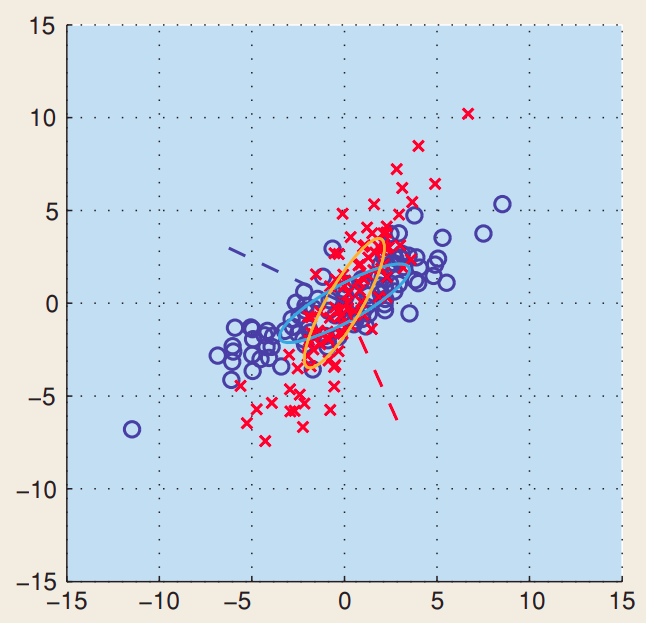
\includegraphics[width=1.\linewidth]{images_report/sensor/before_csp_filtering.png}
        \caption{Before CSP filtering}
        \label{fig:before_csp}
    \end{subfigure}%
    \begin{subfigure}{.5\textwidth}
        \centering
        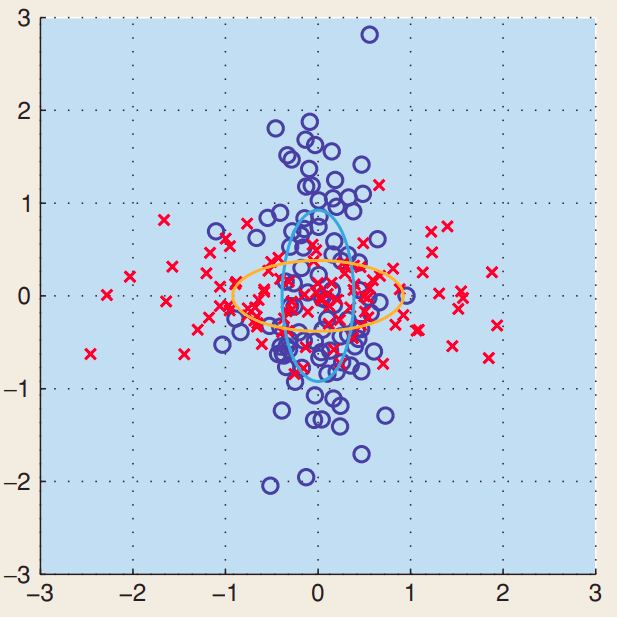
\includegraphics[width=1.\linewidth]{images_report/sensor/after_csp_filtering.png}
        \caption{After CSP filtering}
        \label{fig:after_csp}
    \end{subfigure}
    \caption{Toy example showing the functioning of the CSP transformation.}
    \label{fig:csp_intuitive}
\end{figure}
[je peux faire un shema mieux]

Si on a deux signaux gaussiens, tous les deux centrés en zeros, mais avec des directions principales différentes, on peut tenter de transformer les deux nuages de points de telle manière à ce que les diretions principales des deux nuages de points dans l'espaces des CSP soient orthogonales de façon à maximiser le rapport des variances suivants les directions principales.

On part de deux nuage de points, rouge et bleu, très corrélées, que l'on transforme en des nuages de points rouges' et bleu' découplées.

Par example sur la figure \ref{fig:csp_intuitive}, le vecteur principal du nuage rouge' est aligné sur l'axe des absices, tandis que le vecteur principal du nuage blueu' est aligné sur l'axe des ordonnées.

Par ce procédé, on maximise alors le rapport de variance suivant l'axe des abscices entre le nuage rouge' et le nuage bleu'.


Les nuages de pooints correpondent à un event, et chaque couleur correpond à une condition différente. Si l'on essaye de deviner la couleur/condition d'un nuage de point, il suffit par la suite de transformer le nuage de point avec la même transformation que prescedement, et de prendre la projection sur l'axe des abcices du nuage de point transformé dans l'espace des CSP. On peut alors calculer la variance suivant l'axe des abcises et suivant l'axe des abscice, puis entrainer un classifieru linéaire à disciminer parmis les différentes variances ce qui permet de classifier entre les deux conditions.


Par la suite, on peut entrainer un classifieur linéaire qui prend en entré

\subsubsection{Technical Description}

L'explication prescedente ne fait qu'expliquer intuitivement l'algorithme pour la première composante du CSP. Mais la manière la plus efficace d'implementer les CSP est de formaliser le problème sous la forme d'un problme de vecteur propres generalisé.
[mettre les deux autres formulations]

\paragraph{General Eigenvalue Problem Formulation}

Let $X \in \mathbb{R}^{C * T}$ be a matrix containing  $C$ channels and $T$ time points. The data at a single time point is denoted by $x(t) \in  \mathbb{R}^{C}$. Common spatial pattern (CSP) finds a decomposition that projects the signal in the original sensor space to CSP space using the following transformation:

\begin{equation}
    x_{\text{CSP}}(t) = W^{T}x(t)
\end{equation}

where each column of $W \in \mathbb{R}^{C*C}$ is a spatial filter and each row of $x_{\text{CSP}}(t)$ is a CSP component. Let $\Sigma^{+} \in \mathbb{R}^{C * C}$ and $\Sigma^{-} \in \mathbb{R}^{C * C}$ be the respective covariance matrices of the two differnet  conditions. CSP analysis is given by the simultaneous diagonalization of the two covariance matrices.


\begin{equation}
    W^{T} \Sigma^{+} W = \lambda^{+}
    \label{eq:lambda_plus}
\end{equation}
\begin{equation}
    W^{T} \Sigma^{-} W = \lambda^{-}
    \label{eq:lambda_minus}
\end{equation}

Where the two $\lambda$ are diagonal matrices whose entries are the eigenvalues of the following generalized eigenvalue problem in $(w, \lambda) \in (\mathbb{R}^{C}, \mathbb{R})$:

\begin{equation}
    \Sigma^{+} w = \lambda \Sigma^{-} w
    \label{eq:general_eigenvalue}
\end{equation}

Large entries in the diagonal matrix corresponds to a spatial filter which gives high variance in one class but low variance in the other. Thus, the filter facilitates discrimination between the two classes.

\paragraph{The unmixing matrix}

Une autre manière de lire les deux equations \ref{eq:lambda_plus} et \ref{eq:lambda_minus} est de se rappeller que $w^{T}\Sigma w$ calcule la variance de la covariance $\Sigma$ suivant la direction $w$. Ainsi, $W^{T} \Sigma^{+} W$ et $W^{T} \Sigma^{-} W$ ne font que calculer des matrices diagonales, dont les elements diagonaux sont les variances des covariances suivant les différentes colonnes de $W$, à savoir les variances suivant les difféntes filtres spatiaux.

En trouvant tous les $w$ qui satisfont l'équation \ref{eq:general_eigenvalue}, on construit ainsi la matrice $W$ aussi appellée \textit{unmixing matrix}.

Apres avoir trouvé tous les couples $(w_i, \lambda_i)$ qui satisfont l'équation aux valeurs propres généralisées \ref{eq:general_eigenvalue}, on peut ordonner les solutions par valeurs propres décroissantes. Le premier filtre correspond à la direction maximisant le rapport des variances entre les deux nuages de points. En effet, si l'on remplace dans l'équaqtion \ref{eq:lambda_plus}, \ref{eq:lambda_minus}, on obtient:

\begin{equation}
    w^{T}_{i} \Sigma^{+} w_{i} = \lambda^{+}_{i}
    \label{eq:lambda_plus_first_component}
\end{equation}
\begin{equation}
    w^{T}_{i} \Sigma^{-} w_{i} = \lambda^{-}_{i}
    \label{eq:lambda_minus_first_component}
\end{equation}

Et il suffit alors de remplacer dans \ref{eq:general_eigenvalue} puis de multiplier à gauche par $w^{T}$ pour obtenir

\begin{equation}
    \lambda_1 = \lambda^{+}_1 / \lambda^{-}_1
\end{equation}

% complement eventuel
% https://www.youtube.com/watch?v=S4znknOIcRk&t=332s
% https://www.youtube.com/watch?v=zsOULC16USU

\subsection{Significance of time-frequency bins with Permutation statistics}

We try to answer the following question: is the difference between
the two conditions statistically significant? We use the a permutations
cluster tests on the time-frequency roc-auc map in order to check the significance of the activation.

\subsubsection{Overview of the cluster permutation statistics method}

\begin{figure}[ht]
    \centering
    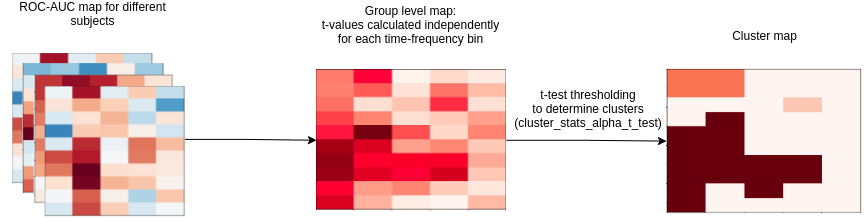
\includegraphics[width=15cm]{images_report/sensor/Permutation_statistics.png}
    \caption[Overview of the permutation statistics pipeline.]%
    {Overview of the permutation statistics pipeline.}
    \label{permutation_statistics_pipeline}
\end{figure}

La figure \ref{permutation_statistics_pipeline} donne un apercut de la pipeline de création des clusters.

On commence par rassembler toutes les time-frequency roc-auc map de tous les sujets. Pour chaque time-frequency bin, on calcule une t-value, de manière indépendante pour chaque bin (le détail des calculs se trouve en annexe). On obtient anisi la carte des t-values. Puis afin de trouver l'emplacement des clusters, il suffit d'utiliser un seiuil, par exemple correspodant à un niveau de chance de $0.05$ ou de $0.01$. Ce seil n'a pas une grande importance mathématique, mais en pratique, il permet de controler la taille des clusters. Une fois le seuil appliqué, on obtient potentiellement un ou des clusters. Afin de pouvoir attribuer une p-valeurs à chaque cluster, il faut alors utiliser le mécanismes des permutations.

Le mécanisme des permutation consiste à caluler une métrique sur nos cluster: qui peut être classiquement soit la taille du cluster, soit le maximum de t-vleur au sein du cluster, soit la somme des t-valeur au sein du cluster. Puis on compare cette métrique à la distribution de cette métrique simulée pour les permutation:
On inverse le signe de la différence pour chaque bin de chaque subject. On obtient la distribution de la metrique dans l'hypothese nulle ou The distribution of spatial cluster sizes is independent of the sign of the data.


\subsection{Implementation}



\subsection{Results}
- Discussion
- resultats significatifs alors que dans la tête


\subsection{Limites + Discu}

- Seuelemnt 2 classes

\section{Source Space}

- Generalités source space
Nouveau script: Contrast in source space
- Motivation : Insuffiscance de pipeline classique
- faire le Schéma
- Results:
- Interpretation sur Freeview
- Discussion
- Annexes : Subtilité :
Neuroscience : quest ce qui constitue du bruit ? Quel choix de la matrice de covariance
Subtilités mathématiques :  commutativité Log + moyenne
Limites:
